\chapter{Desarrollo del software}

En este capítulo se describe el desarrollo de la aplicación. En primer lugar se analizan las
arquitecturas y patrones de diseño que fundamentan la solución. A continuación se documentan los
\textit{sprints} realizados, siguiendo para cada uno el mismo esquema: diseño de la interfaz, diseño
de los datos, diseño del software, implementación y pruebas.

\section{Análisis de arquitecturas y patrones}

El sistema debe transformar dos fuentes de datos (un fichero de nodos y una matriz de adyacencia)
en una representación 3D interactiva navegable en tiempo real desde el navegador. Esta
transformación se puede entender como una \textit{tubería de procesamiento y visualización}: los
datos se leen y validan, se convierten en un grafo, se exponen mediante una API y se renderizan en
el cliente. Cualquier error en la etapa de datos se propaga al renderizado final, por lo que la
robustez del parseo y la validación es un aspecto crítico.

Para reducir la variabilidad del entorno y facilitar el mantenimiento, se ha optado por una
\textbf{arquitectura cliente-servidor desacoplada}, organizada en dos servicios independientes
comunicados a través de una API REST:

\begin{itemize}
	\item \textbf{Backend (servicio de datos y análisis).} Implementado en Python con Flask. Se
		encarga de leer los ficheros, construir el grafo con NetworkX, calcular las métricas y
		exponer la red en formato JSON. Sigue un enfoque minimalista, orientado exclusivamente a
		servir datos.
	\item \textbf{Frontend (aplicación cliente).} Implementado en React con Three.js a través de
		\textit{react-three-fiber}. Consume la API y gestiona la visualización 3D y el estado de la
		interfaz.
\end{itemize}

Ambos servicios se empaquetan en \textbf{contenedores Docker}~\cite{docker} y se orquestan con
Docker Compose, lo que garantiza un despliegue reproducible con independencia del sistema operativo
anfitrión. El
navegador se comunica únicamente con el frontend; las peticiones a la API se redirigen
internamente al backend dentro de la red de contenedores mediante un \textit{proxy}. La
figura~\ref{fig:arquitectura} resume esta arquitectura general.

\begin{figure}[H]
	\centering
	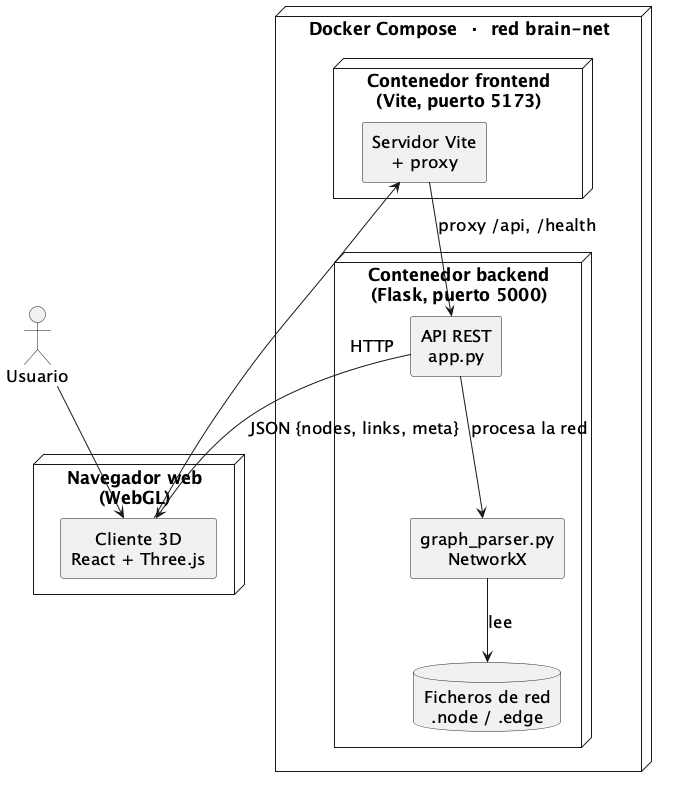
\includegraphics[height=12.5cm]{imagenes/arquitectura}
	\caption{Arquitectura general del sistema.}
	\label{fig:arquitectura}
\end{figure}

En cuanto a los \textbf{patrones de diseño}, la solución se apoya en:

\begin{itemize}
	\item \textbf{Separación de responsabilidades} entre procesamiento de datos (backend) y
		presentación (frontend).
	\item \textbf{Modelo declarativo basado en componentes} en el frontend, propio de React, que
		permite describir la escena 3D y los paneles de la interfaz como componentes reutilizables.
	\item \textbf{Gestión de estado unidireccional} mediante los \textit{hooks} de React, de forma
		que los cambios en los controles (por ejemplo, el umbral de filtrado) se propagan de manera
		predecible a la escena.
\end{itemize}

Durante el análisis se identificaron algunos riesgos técnicos que han condicionado estas
decisiones: la sobrecarga visual por exceso de aristas, la inconsistencia de formatos en los
ficheros de entrada, posibles cuellos de botella en el renderizado y la dependencia del entorno
local. La arquitectura desacoplada y el despliegue con contenedores mitigan principalmente los dos
últimos.

\section{Sprint 1}

El primer \textit{sprint} corresponde a los requisitos de \textbf{Prioridad 1} (RF 1 a RF 4) y
constituye el producto mínimo viable (MVP) de la aplicación. Su objetivo es que un visitante pueda,
sin registro ni instalación de ningún tipo, cargar una red cerebral, procesarla en el \textit{backend}
y visualizarla en 3D, navegando por la escena con la cámara y consultando un panel con las
estadísticas globales de la red.

Al ser el primer \textit{sprint}, además de la funcionalidad propia se ha llevado a cabo toda la
puesta a punto del proyecto: la definición de la arquitectura cliente-servidor, la creación de los
dos servicios (\textit{backend} y \textit{frontend}), la definición del contrato de la API que los
comunica y la configuración del entorno de ejecución con contenedores. Por ello, este \textit{sprint}
sienta las bases técnicas sobre las que se construirán todos los siguientes. En los apartados
siguientes se detalla el diseño de la interfaz, el diseño de los datos, el diseño del software, la
implementación realizada y las pruebas con las que se ha validado.

\subsection{Diseño de la interfaz}

Antes de implementar la interfaz se elaboró un \textbf{boceto (\textit{mockup})} de su distribución,
que sirvió de guía para el desarrollo. La interfaz se ha diseñado como una \textbf{aplicación de una
sola pantalla} en la que la escena 3D ocupa todo el espacio disponible y la información se superpone
en paneles (HUD) situados en las esquinas, de modo que no obstruyan la visualización. Los elementos
principales, mostrados en el \textit{mockup} de la figura~\ref{fig:mockup}, son:

\begin{itemize}
	\item El \textbf{lienzo 3D} central con la red renderizada.
	\item Un \textbf{panel superior izquierdo} con la identidad de la aplicación y las estadísticas
		globales (nodos, conexiones, grupos).
	\item Un \textbf{panel superior derecho} con los controles de visualización.
	\item Una \textbf{leyenda} en la esquina inferior izquierda con la correspondencia entre colores
		y grupos.
\end{itemize}

Se opta por una línea sobria y minimalista: superficies planas, tipografía clara, líneas finas y un
único color de acento, de modo que la atención recaiga sobre la visualización de la red y no sobre
los adornos de la propia interfaz. En este \textit{sprint} no se incluye ninguna pantalla de acceso,
ya que la gestión de usuarios corresponde al Sprint 4.

\begin{figure}[H]
	\centering
	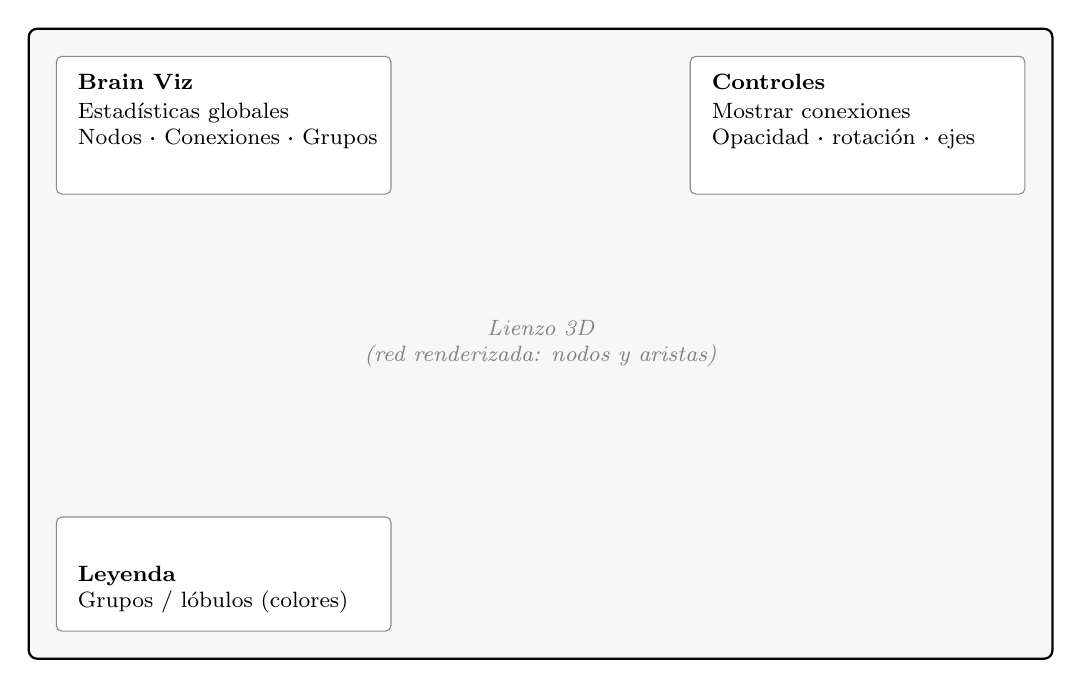
\begin{tikzpicture}[font=\footnotesize]
		% Marco de la pantalla
		\draw[rounded corners=3pt, thick, fill=black!3] (0,0) rectangle (13,8);
		% Etiqueta central de la escena 3D
		\node[align=center, gray] at (6.5,4) {\itshape Lienzo 3D\\\itshape (red renderizada:
		nodos y aristas)};
		% Panel superior izquierdo: identidad + estadísticas
		\draw[rounded corners=2pt, fill=white, draw=black!45] (0.35,5.9) rectangle (4.6,7.65);
		\node[anchor=north west, align=left] at (0.5,7.55)
			{\textbf{Brain Viz}\\[1pt]\footnotesize Estadísticas globales\\\footnotesize Nodos ·
			Conexiones · Grupos};
		% Panel superior derecho: controles
		\draw[rounded corners=2pt, fill=white, draw=black!45] (8.4,5.9) rectangle (12.65,7.65);
		\node[anchor=north west, align=left] at (8.55,7.55)
			{\textbf{Controles}\\[1pt]\footnotesize Mostrar conexiones\\\footnotesize Opacidad ·
			rotación · ejes};
		% Leyenda inferior izquierda
		\draw[rounded corners=2pt, fill=white, draw=black!45] (0.35,0.35) rectangle (4.6,1.8);
		\node[anchor=south west, align=left] at (0.5,0.45)
			{\textbf{Leyenda}\\\footnotesize Grupos / lóbulos (colores)};
	\end{tikzpicture}
	\caption{Boceto (\textit{mockup}) de la distribución de la interfaz principal.}
	\label{fig:mockup}
\end{figure}

\subsection{Diseño de los datos}

Los datos de entrada siguen el formato de \textit{BrainNet Viewer}, descrito en los requisitos de
información [RI 1, RI 2]:

\begin{itemize}
	\item El fichero \texttt{.node} contiene una fila por nodo con las columnas
		\texttt{x  y  z  color\_id  size  label}.
	\item El fichero \texttt{.edge} contiene la matriz de adyacencia $N \times N$ con los pesos de
		las conexiones.
\end{itemize}

La red de ejemplo empleada en este \textit{sprint} es \textbf{AAL90}~\cite{aal}, una parcelación del
cerebro en 90 regiones anatómicas. Su fichero \texttt{.node} contiene, por tanto, 90 filas (una por
región, con sus coordenadas, su lóbulo y su etiqueta) y su fichero \texttt{.edge} una matriz de
adyacencia de $90 \times 90$ con los pesos de conectividad entre cada par de regiones.

\textbf{Almacenamiento en el servidor.} En este primer \textit{sprint} el sistema \textit{no utiliza
base de datos}: las redes públicas precargadas se almacenan directamente como los ficheros
\texttt{.node} y \texttt{.edge} en el servidor. La persistencia mediante base de datos ---necesaria
para las cuentas de usuario y los conjuntos de datos privados, descrita en el requisito de
información [RI 4]--- se introducirá en el Sprint 4, junto con la gestión de usuarios.

\textbf{Modelo interno.} El sistema transforma estas dos fuentes de datos en un modelo interno que no
es un fichero ni una base de datos, sino una \textbf{estructura de datos en memoria}: un grafo (objeto
de la librería de análisis) construido a partir de la matriz de adyacencia, en el que cada nodo se
enriquece con sus coordenadas espaciales, su etiqueta y su grupo. Este grafo es transitorio: existe
únicamente durante el procesamiento de la petición. Como decisión de diseño para reducir la sobrecarga
visual, las aristas cuyo peso es inferior a un umbral mínimo se descartan en esta primera versión, de
modo que solo se representan las conexiones relevantes.

Tras el procesamiento, el \textit{backend} expone la red al \textit{frontend} mediante una estructura
JSON acordada como contrato de la API, con tres bloques:
\begin{itemize}
	\item \texttt{nodes}: lista de nodos, cada uno con su identificador, su etiqueta, sus coordenadas
		$(x, y, z)$ y su grupo o lóbulo.
	\item \texttt{links}: lista de conexiones, cada una con el nodo origen, el nodo destino y el peso
		de la conexión.
	\item \texttt{meta}: metadatos globales de la red, con el número total de nodos y de aristas.
\end{itemize}
Este formato es ligero y directo de consumir por el \textit{frontend}, que lo utiliza tanto para
construir la geometría 3D como para alimentar el panel de estadísticas.

\subsection{Diseño del software}

El backend se organiza en torno a dos módulos principales: un módulo de parseo, responsable de
leer los ficheros, construir el grafo con NetworkX y generar la estructura JSON, y un módulo de
aplicación que define los \textit{endpoints} de la API. La siguiente tabla resume ambos módulos.

\begin{table}[H]
	\centering
	\caption{Módulos del backend en el Sprint 1.}
	\begin{tabularx}{\textwidth}{>{\raggedright\arraybackslash}p{3.2cm} >{\raggedright\arraybackslash}X}
		\toprule
		\textbf{Módulo} & \textbf{Responsabilidad} \\
		\midrule
		\texttt{graph\_parser} & Lee los ficheros \texttt{.node} y \texttt{.edge}, valida su
			consistencia, construye el grafo con NetworkX y genera la estructura JSON de la red. \\
		\addlinespace
		\texttt{app} & Define la aplicación Flask y los \textit{endpoints} de la API
			(\texttt{/health} y \texttt{/api/brain-data}). \\
		\bottomrule
	\end{tabularx}
\end{table}

Los \textit{endpoints} disponibles en este \textit{sprint} son \texttt{/health}, para la
verificación del estado del servicio, y \texttt{/api/brain-data}, que devuelve la red procesada.

En el \textit{frontend}, la aplicación se estructura en componentes siguiendo el modelo declarativo
de React. El componente raíz mantiene el estado global de la interfaz (los metadatos de la red, el
nodo sobre el que se sitúa el cursor y los ajustes de visualización) y contiene la escena 3D y los
paneles del HUD. Un componente de visualización independiente es el encargado de solicitar los datos
a la API y de generar la geometría de nodos y aristas a partir de ellos. La comunicación entre
controles y escena es unidireccional: cuando el usuario modifica un ajuste (por ejemplo, la opacidad
de las aristas), el cambio se propaga desde el estado hacia la escena, que se vuelve a dibujar de
forma reactiva. La figura~\ref{fig:modulos} muestra la modularización del software en este
\textit{sprint}.

\begin{figure}[H]
	\centering
	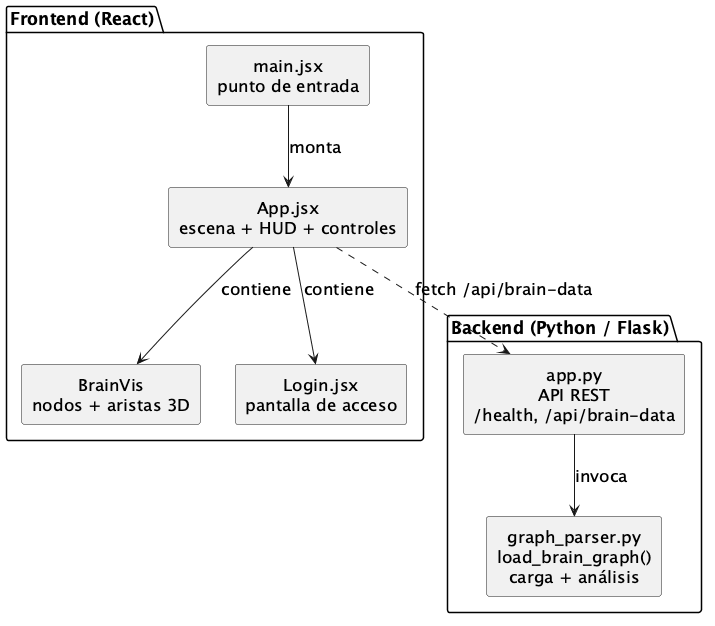
\includegraphics[height=10cm]{imagenes/modulos_sprint1}
	\caption{Modularización del software en el Sprint 1.}
	\label{fig:modulos}
\end{figure}

El modelo de dominio del \textit{backend} se organiza en torno a una clase principal,
\texttt{BrainNetwork}, que representa la red procesada y se compone de sus \texttt{Node}s, sus
\texttt{Edge}s y un bloque de metadatos (\texttt{Meta}). La clase \texttt{GraphParser} es la
responsable de construir esa red a partir de los ficheros de entrada, y la clase \texttt{BrainVizApi}
la expone a través de los \textit{endpoints} de la API. La figura~\ref{fig:clases} recoge este
diagrama de clases (con la nomenclatura en inglés, coherente con la del código).

\begin{figure}[H]
	\centering
	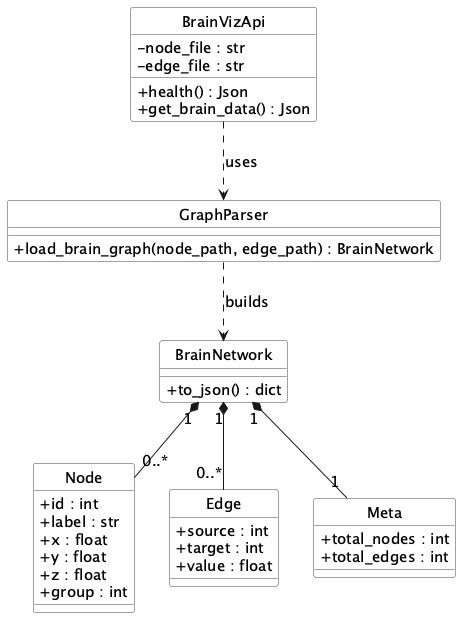
\includegraphics[height=9.5cm]{imagenes/clases_sprint1}
	\caption{Diagrama de clases del modelo de dominio del backend (Sprint 1).}
	\label{fig:clases}
\end{figure}

El flujo de la carga inicial de la red es el siguiente: al abrir la aplicación, el frontend realiza
una petición a \texttt{/api/brain-data}; el backend lee los ficheros de la red, construye el grafo,
lo serializa a JSON y lo devuelve; el frontend recibe los datos, calcula la geometría y renderiza la
escena, actualizando además el panel de estadísticas. Este flujo se representa en el diagrama de
secuencia de la figura~\ref{fig:secuencia}.

\begin{figure}[H]
	\centering
	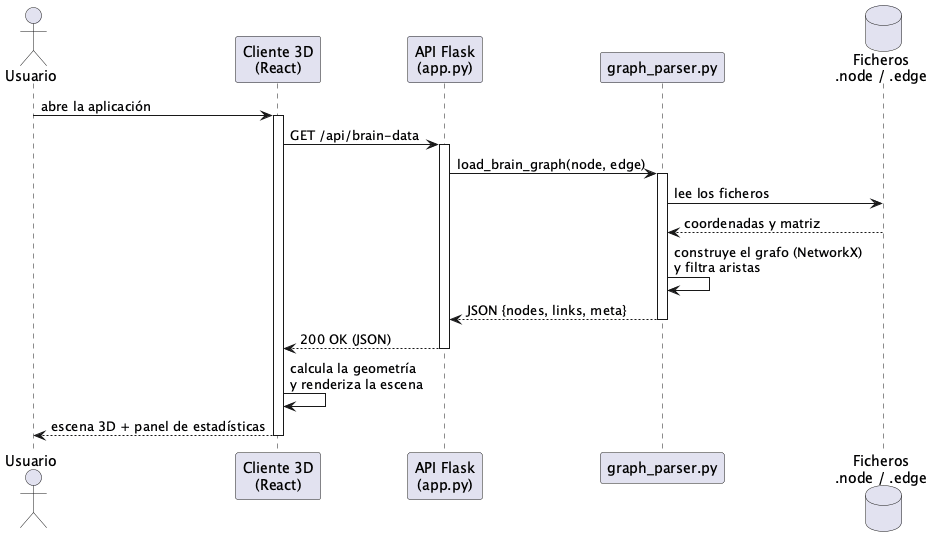
\includegraphics[width=\textwidth]{imagenes/sec_carga_red}
	\caption{Diagrama de secuencia de la carga y visualización de una red.}
	\label{fig:secuencia}
\end{figure}

Conviene señalar una limitación de este diseño inicial: tal y como está planteado, cada petición de
una red reconstruye el grafo y su JSON desde los ficheros, de modo que visualizar la misma red muchas
veces repite el mismo trabajo. Para las redes públicas, que no cambian, esto es ineficiente. Una
mejora prevista ---que se abordará al introducir la persistencia en el Sprint 4--- es \textbf{construir
la red y su JSON una sola vez y almacenar el resultado} (en una caché o en la base de datos) para
reutilizarlo en las siguientes peticiones, evitando así el reprocesamiento.

\subsection{Implementación}

La implementación de este \textit{sprint} cubre los requisitos de Prioridad 1 (RF 1 a RF 4) y se
reparte entre los dos servicios de la aplicación, el \textit{backend} y el \textit{frontend}, más la
configuración del entorno de despliegue. A continuación se detalla el trabajo realizado en cada uno.

\subsubsection*{Backend: procesamiento y API (RF 1, RF 2.1)}

El \textit{backend} se ha implementado en Python con Flask y se organiza en los dos módulos descritos
anteriormente. El módulo de parseo es el núcleo del procesamiento y realiza la siguiente secuencia de
tareas:

\begin{enumerate}
	\item \textbf{Validación de entrada.} Comprueba que existen los ficheros de nodos y de aristas y,
		en caso contrario, informa del error sin que el servicio se detenga.
	\item \textbf{Lectura de los datos.} Lee el fichero de nodos como una tabla, admitiendo tanto
		espacios como tabuladores como separadores, y carga la matriz de adyacencia.
	\item \textbf{Construcción del grafo.} Convierte la matriz de adyacencia en un grafo no dirigido
		mediante NetworkX y asocia a cada nodo sus atributos (coordenadas, etiqueta y grupo).
	\item \textbf{Filtrado de aristas.} Descarta las conexiones con un peso por debajo del umbral
		mínimo, para no saturar la visualización con enlaces poco significativos.
	\item \textbf{Serialización.} Genera la estructura JSON con los bloques \texttt{nodes},
		\texttt{links} y \texttt{meta} que consume el \textit{frontend}.
\end{enumerate}

El núcleo de este procesamiento es breve gracias a NetworkX. El siguiente fragmento resume la
construcción del grafo a partir de la matriz de adyacencia y el filtrado de aristas por umbral:

\begin{lstlisting}[language=Python, basicstyle=\footnotesize\ttfamily, keywordstyle=\color{blue!60!black}, commentstyle=\color{gray}, showstringspaces=false, frame=single, columns=fullflexible]
# Grafo no dirigido a partir de la matriz de adyacencia
G = nx.from_numpy_array(adj_matrix, create_using=nx.Graph)

# Filtrado de aristas por umbral y serializacion a JSON
links = [
    {"source": u, "target": v, "value": w}
    for u, v, w in G.edges.data("weight")
    if w > THRESHOLD
]
\end{lstlisting}

El uso de NetworkX en esta fase, aunque en el Sprint 1 se limita a la construcción del grafo, deja
preparada la infraestructura para el cálculo de métricas de teoría de grafos en los \textit{sprints}
posteriores. Sobre este módulo, la aplicación Flask define los dos \textit{endpoints} de la API.
Además de responder en JSON, ambos incorporan una negociación de contenido que permite devolver una
página HTML legible cuando se accede a ellos desde el navegador, lo que facilita la depuración durante
el desarrollo. La comunicación con el \textit{frontend} se habilita mediante CORS.

\subsubsection*{Frontend: visualización e interacción (RF 2, RF 3, RF 4)}

El \textit{frontend} se ha implementado en React con Vite como herramienta de construcción, y utiliza
Three.js a través de \textit{react-three-fiber} y su librería de utilidades \textit{drei} para el
renderizado 3D declarativo. Al iniciarse, la aplicación solicita la red al \textit{endpoint}
\texttt{/api/brain-data} y, con los datos recibidos, construye la escena:

\begin{itemize}
	\item \textbf{Nodos (RF 2).} Cada nodo se representa como una esfera situada en sus coordenadas
		anatómicas, coloreada según su grupo o lóbulo mediante una paleta categórica, de forma que las
		regiones de una misma agrupación comparten color.
	\item \textbf{Aristas (RF 2).} Las conexiones se dibujan como segmentos de línea entre los nodos
		que unen. Su opacidad es ajustable, lo que permite atenuarlas para percibir mejor la estructura
		en redes densas.
	\item \textbf{Navegación (RF 3).} La cámara se controla con los controles de órbita de Three.js,
		que permiten rotar, hacer zoom y desplazar la escena, con amortiguación para un movimiento
		suave y límites de acercamiento y alejamiento para no perder el modelo de vista.
	\item \textbf{Panel de estadísticas (RF 4).} Un panel superpuesto (HUD) muestra en tiempo real el
		número de nodos, de conexiones y de grupos de la red activa.
\end{itemize}

La interfaz se completa con un panel de controles de visualización (mostrar u ocultar las conexiones,
activar la rotación automática de la escena, mostrar los ejes de referencia y ajustar la opacidad de
las aristas mediante un deslizador), una leyenda que asocia cada color a su grupo, la información
emergente al situar el cursor sobre un nodo y unos estados de carga y de error que informan al usuario
mientras se obtienen los datos o si estos no están disponibles. Todo ello sigue una línea visual sobria
y minimalista, coherente con la naturaleza científica de la herramienta.

\subsection{Despliegue y control de versiones}

Ambos servicios se han contenerizado y se orquestan con Docker Compose, que los levanta en una red
interna común. El navegador solo se comunica con el \textit{frontend}, y las peticiones a la API se
redirigen internamente al \textit{backend} mediante un \textit{proxy}, evitando así problemas de
CORS y de configuración de puertos en el cliente. El entorno está preparado para el desarrollo con
recarga en caliente, de modo que los cambios en el código se reflejan de inmediato sin reconstruir las
imágenes. El detalle del procedimiento de instalación y ejecución se recoge en el manual de
instalación.

El desarrollo se ha gestionado con control de versiones mediante Git, alojando el repositorio en
GitHub y registrando el avance con \textit{commits} sucesivos a lo largo del \textit{sprint}. El
código completo puede consultarse en el repositorio público del proyecto:
\url{https://github.com/pablomlz/brain-viz}.

\subsection{Pruebas}

La estrategia de pruebas de cada \textit{sprint} combina tres tipos de pruebas: pruebas de caja
blanca (unitarias) sobre el código, pruebas de caja negra (de integración) sobre la comunicación
entre servicios y pruebas de validación (o de aceptación) que comprueban el cumplimiento de los
requisitos. Conviene recordar que, en ingeniería del software, una prueba se considera exitosa
cuando es capaz de \emph{descubrir un error}; por ello, al final de este apartado se describen
algunos de los errores detectados y cómo se corrigieron.

\subsubsection*{Pruebas de caja blanca (unitarias)}

Se han probado de forma aislada las funciones del módulo de parseo, comprobando que, ante ficheros
correctos, el grafo resultante tiene el número esperado de nodos y aristas y que los atributos de los
nodos (coordenadas, etiqueta y grupo) se corresponden con los del fichero de entrada. También se han
probado los casos límite: ficheros inexistentes, matriz de adyacencia con dimensiones que no
coinciden con el número de nodos y valores fuera de rango.

\subsubsection*{Pruebas de caja negra (de integración)}

Se ha verificado la comunicación entre el \textit{frontend} y el \textit{backend} a través de la API,
sin conocer la implementación interna: se comprueba que el \textit{endpoint} \texttt{/api/brain-data}
responde con un JSON cuya estructura respeta el contrato acordado (\texttt{nodes}, \texttt{links} y
\texttt{meta}) y que el \textit{frontend} es capaz de renderizar la escena a partir de esa respuesta.

\subsubsection*{Pruebas de validación (de aceptación)}

Por último, se han diseñado pruebas de validación alineadas con los criterios del capítulo de
requisitos, que verifican que cada requisito de Prioridad~1 se comporta como se espera. La
tabla~\ref{tab:pruebas} recoge estas pruebas, el requisito que validan y su resultado.

\begin{table}[H]
	\centering
	\caption{Pruebas de validación del Sprint 1.}
	\label{tab:pruebas}
	\small
	\begin{tabularx}{\textwidth}{>{\raggedright\arraybackslash}p{1.4cm} >{\raggedright\arraybackslash}X >{\raggedright\arraybackslash}X >{\centering\arraybackslash}p{1.6cm}}
		\toprule
		\textbf{Prueba} & \textbf{Descripción} & \textbf{Resultado esperado} & \textbf{Estado} \\
		\midrule
		P-01 (RF 2.1) & Petición a \texttt{/health} y a \texttt{/api/brain-data}. &
			\texttt{/health} responde \texttt{ok}; \texttt{/api/brain-data} devuelve un JSON válido
			con \texttt{nodes}, \texttt{links} y \texttt{meta}. & Correcto \\
		\addlinespace
		P-02 (RF 1, RF 2) & Carga y renderizado del atlas AAL90. &
			Los 90 nodos se sitúan en sus coordenadas y las aristas conectan los nodos correctos. &
			Correcto \\
		\addlinespace
		P-03 (RF 2.1) & Carga con ficheros de dimensiones incongruentes. &
			El sistema detecta el error y no cae (respuesta de error controlada). & Correcto \\
		\addlinespace
		P-04 (RF 3) & Navegación con la cámara (rotar, zoom y paneo). &
			La cámara responde de forma fluida, con amortiguación y límites de zoom. & Correcto \\
		\addlinespace
		P-05 (RF 4) & Comprobación del panel de estadísticas. &
			El HUD muestra el número de nodos, aristas y grupos coherente con los datos de entrada. &
			Correcto \\
		\bottomrule
	\end{tabularx}
\end{table}

\subsubsection*{Errores detectados y corregidos}

Durante las pruebas se detectaron y corrigieron varios errores, lo que confirma su utilidad. Los más
relevantes fueron:

\begin{itemize}
	\item \textbf{Etiqueta incorrecta en la información del nodo.} Al situar el cursor sobre un nodo, la
		información emergente mostraba un texto genérico (``Nodo \#\textit{i}'') en lugar del nombre de
		la región. La prueba de la interacción reveló que el código leía un campo inexistente
		(\texttt{name}) en vez del campo real del contrato de la API (\texttt{label}); se corrigió
		haciendo que leyera \texttt{label}.
	\item \textbf{Caída ante ficheros incongruentes.} Una primera versión no comprobaba que las
		dimensiones de la matriz de adyacencia coincidieran con el número de nodos, lo que provocaba un
		error no controlado. La prueba de caja blanca con ficheros incongruentes lo puso de manifiesto
		y se añadió la validación correspondiente, que ahora devuelve un error controlado [RNF 3].
\end{itemize}

Estas pruebas se han realizado de forma manual sobre el entorno desplegado con contenedores. En los
sucesivos \textit{sprints} se completarán con pruebas automatizadas del \textit{backend} y con la
medición del rendimiento gráfico (FPS) para verificar el requisito no funcional de fluidez [RNF 1].

\subsubsection*{Validación por parte del cliente}

Al finalizar el \textit{sprint} se realiza la prueba fundamental de todo desarrollo ágil: la
validación por parte del cliente, cuyo papel asume el director del proyecto. Para que pueda probar la
aplicación de forma cómoda ---y, más adelante, también el tribunal---, el Sprint~1 se despliega en un
servidor público accesible y se le facilita su URL.
% NOTA: insertar aquí la URL del despliegue una vez publicado el Sprint 1 en el servidor.

\section{Sprint 2}

El segundo \textit{sprint} corresponde a los requisitos de \textbf{Prioridad 2} (RF 5, RF 6 y RF 7) y
constituye el núcleo de la exploración interactiva de la red. Mientras que el Sprint~1 permitía
\emph{ver} la red, este \textit{sprint} permite \emph{explorarla}: reducir su complejidad visual
filtrando las conexiones menos relevantes (RF 5), consultar la información concreta de una región
seleccionándola con el ratón (RF 6) y distinguir las agrupaciones anatómicas mediante el coloreado y
su leyenda (RF 7).

De los tres requisitos, el RF 7 ya quedó cubierto durante el Sprint~1, puesto que el coloreado por
grupo y su leyenda eran necesarios para que la visualización inicial resultara legible; en este
\textit{sprint} se da por consolidado y el esfuerzo se concentra en los otros dos. El desarrollo ha
requerido modificar tanto el \textit{backend} ---que hasta ahora aplicaba un umbral fijo y no
proporcionaba toda la información de cada nodo--- como el \textit{frontend}, donde reside la
interacción.

\subsection{Diseño de la interfaz}

El diseño parte del establecido en el Sprint~1 y añade dos elementos, manteniendo el principio de que
la escena 3D ocupe todo el espacio y la información se superponga en paneles que no la obstruyan:

\begin{itemize}
	\item Un \textbf{control deslizante de umbral} en el panel de controles (RF 5). Se sitúa en primer
		lugar por ser el control con mayor impacto sobre la visualización, y muestra junto a él el valor
		numérico del umbral activo.
	\item Un \textbf{panel de información del nodo seleccionado} (RF 6), que aparece bajo el panel de
		controles únicamente cuando hay un nodo seleccionado y puede cerrarse explícitamente. Se ha
		optado por un panel lateral persistente, en lugar de una ventana emergente, para que el usuario
		pueda seguir rotando la escena mientras consulta los datos de la región.
\end{itemize}

Además, el contador de conexiones del panel de estadísticas pasa a mostrar la relación
\textit{visibles / totales}, de modo que el usuario perciba en todo momento qué proporción de la red
está viendo. La figura~\ref{fig:mockup-s2} recoge el boceto de la interfaz resultante, con los dos
elementos nuevos destacados.

\begin{figure}[H]
	\centering
	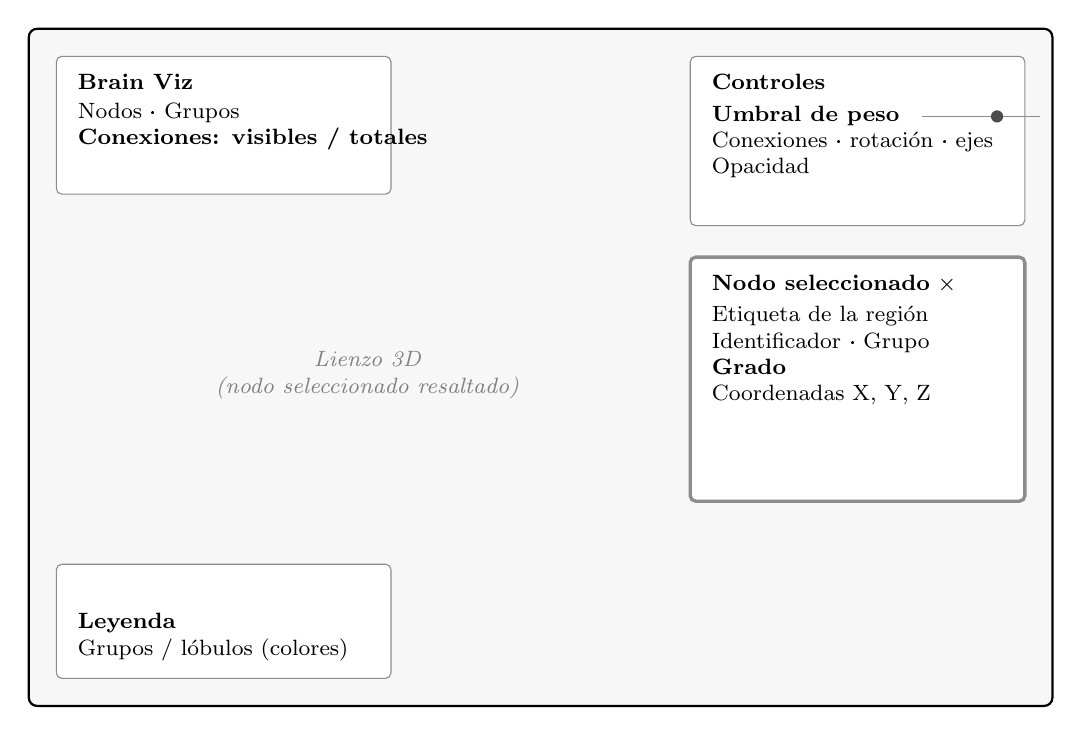
\begin{tikzpicture}[font=\footnotesize]
		% Marco de la pantalla
		\draw[rounded corners=3pt, thick, fill=black!3] (0,0) rectangle (13,8.6);
		% Escena 3D
		\node[align=center, gray] at (4.3,4.2) {\itshape Lienzo 3D\\\itshape (nodo seleccionado
		\itshape resaltado)};
		% Panel superior izquierdo: estadísticas
		\draw[rounded corners=2pt, fill=white, draw=black!45] (0.35,6.5) rectangle (4.6,8.25);
		\node[anchor=north west, align=left] at (0.5,8.15)
			{\textbf{Brain Viz}\\[1pt]\footnotesize Nodos · Grupos\\\footnotesize
			\textbf{Conexiones: visibles / totales}};
		% Panel superior derecho: controles (con umbral destacado)
		\draw[rounded corners=2pt, fill=white, draw=black!45] (8.4,6.1) rectangle (12.65,8.25);
		\node[anchor=north west, align=left] at (8.55,8.15)
			{\textbf{Controles}\\[2pt]\footnotesize\textbf{Umbral de peso} \; \tikz[baseline=-0.5ex]{
				\draw[black!45] (0,0) -- (1.5,0); \fill[black!70] (0.95,0) circle (2.2pt);}\\
			\footnotesize Conexiones · rotación · ejes\\\footnotesize Opacidad};
		% Panel derecho: nodo seleccionado (nuevo)
		\draw[rounded corners=2pt, fill=white, draw=black!45, very thick] (8.4,2.6) rectangle (12.65,5.7);
		\node[anchor=north west, align=left] at (8.55,5.6)
			{\textbf{Nodo seleccionado} \hfill $\times$\\[2pt]\footnotesize Etiqueta de la región\\
			\footnotesize Identificador · Grupo\\\footnotesize \textbf{Grado}\\
			\footnotesize Coordenadas X, Y, Z};
		% Leyenda inferior izquierda
		\draw[rounded corners=2pt, fill=white, draw=black!45] (0.35,0.35) rectangle (4.6,1.8);
		\node[anchor=south west, align=left] at (0.5,0.45)
			{\textbf{Leyenda}\\\footnotesize Grupos / lóbulos (colores)};
	\end{tikzpicture}
	\caption{Boceto de la interfaz del Sprint 2. En trazo grueso, el nuevo panel de información del
	nodo seleccionado; en el panel de controles se incorpora el umbral de peso.}
	\label{fig:mockup-s2}
\end{figure}

\subsection{Diseño de los datos}

Las dos funcionalidades de este \textit{sprint} obligan a revisar el contrato de la API definido en
el Sprint~1, ya que la información que enviaba el servidor resultaba insuficiente:

\begin{itemize}
	\item \textbf{La red debe enviarse completa.} En el Sprint~1 el servidor descartaba las aristas
		por debajo de un umbral fijo. Si el umbral pasa a ser del usuario, el servidor no puede decidir
		de antemano qué aristas sobran: debe enviar todas las conexiones existentes y dejar el filtrado
		al cliente. En la red de ejemplo esto supone pasar de 365 a 411 aristas.
	\item \textbf{Cada nodo incorpora su grado} (\texttt{degree}), es decir, su número de conexiones en
		la red completa. Es un dato que el panel de información debe mostrar (RF 6) y que se calcula en
		el servidor con la librería de análisis de grafos, evitando que el cliente tenga que recorrer
		toda la lista de aristas.
	\item \textbf{Los metadatos incorporan el rango de pesos} (\texttt{min\_weight} y
		\texttt{max\_weight}). Con ellos, el control de umbral se calibra con los pesos reales de la red
		en lugar de asumir un rango fijo, de modo que la interfaz funcione igual con una red cuyos pesos
		sean correlaciones en $[0,1]$ que con otra cuyos valores sean, por ejemplo, recuentos de fibras
		de orden muy distinto. La interfaz muestra además los extremos del rango junto al control, para
		que el usuario sepa entre qué valores se mueve la red que está explorando.
	\item \textbf{Las aristas se envían ordenadas por peso descendente.} Esta decisión, que no altera
		la información transmitida, es la que permite implementar el filtrado de forma eficiente, como
		se explica en el diseño del software.
\end{itemize}

Un matiz importante del modelo de datos es que ahora se distingue entre \emph{existir} y \emph{ser
visible}: una arista existe si su peso es mayor que cero en la matriz de adyacencia ---y como tal
cuenta para el grado de los nodos---, mientras que su visibilidad depende del umbral que fije el
usuario en cada momento. Por ello, el grado que muestra el panel de información se refiere siempre a
la red completa y no varía al mover el control de umbral. La figura~\ref{fig:clases-s2} recoge el
modelo de datos resultante, con los atributos añadidos en este \textit{sprint} destacados.

\begin{figure}[H]
	\centering
	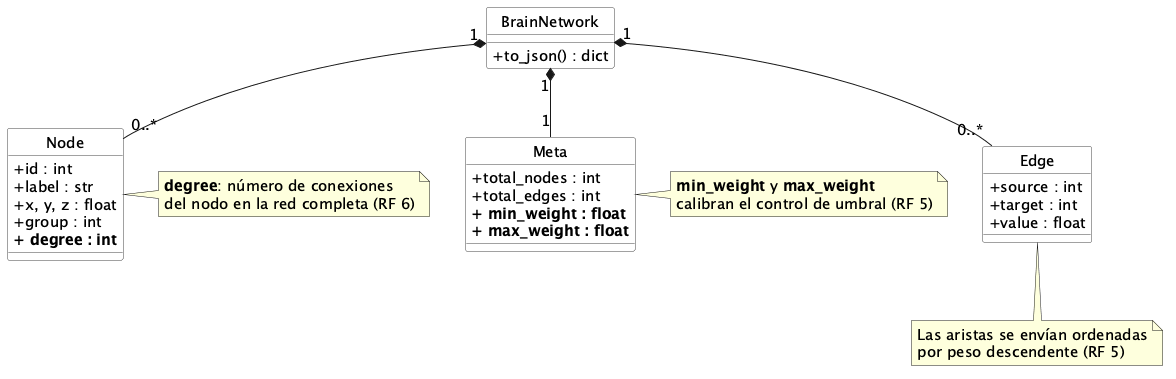
\includegraphics[width=\textwidth]{imagenes/clases_sprint2}
	\caption{Modelo de datos tras el Sprint 2, con los atributos añadidos para el filtrado (RF 5) y la
	inspección de nodos (RF 6).}
	\label{fig:clases-s2}
\end{figure}

\subsection{Diseño del software}

La característica que define este \textit{sprint} desde el punto de vista del diseño es que
\textbf{ninguna de las dos interacciones requiere comunicarse con el servidor}. Tanto el filtrado
como la selección operan sobre los datos que el cliente ya ha recibido, lo que resulta imprescindible
para cumplir el requisito de que el filtrado se aplique \emph{en tiempo real} (RF 5): una petición
por cada movimiento del control deslizante haría la interacción inviable.

El punto delicado es cómo aplicar el umbral sin penalizar el rendimiento. La solución directa
---recorrer las aristas y reconstruir la geometría cada vez que el usuario mueve el control--- obliga
a recalcular y volver a enviar a la tarjeta gráfica miles de vértices en cada fotograma. En su lugar
se ha adoptado la siguiente estrategia, apoyada en que el servidor entrega las aristas ordenadas por
peso descendente:

\begin{enumerate}
	\item La geometría de las aristas se construye \textbf{una sola vez} al cargar la red, con todas
		las conexiones y en orden de peso decreciente.
	\item Al fijar un umbral, las aristas que lo superan son necesariamente las \textbf{primeras} de
		esa secuencia ordenada. Determinar cuántas son se reduce entonces a localizar la posición de la
		primera arista que no alcanza el umbral, lo que se resuelve con una \textbf{búsqueda binaria},
		de coste $O(\log E)$ sobre el número de aristas $E$, en lugar de recorrer la lista completa.
	\item Basta entonces con indicar al motor gráfico cuántos elementos debe dibujar
		(\textit{rango de dibujado}), operación de \textbf{coste constante} que no modifica la
		geometría ni vuelve a enviarla a la tarjeta gráfica.
\end{enumerate}

De este modo, mover el control deslizante no implica reconstruir nada: su coste es logarítmico en el
número de aristas y prácticamente independiente del tamaño de la red, por lo que la escena responde
de forma inmediata. La figura~\ref{fig:sec-s2} muestra el diagrama de secuencia de ambas
interacciones.

\begin{figure}[H]
	\centering
	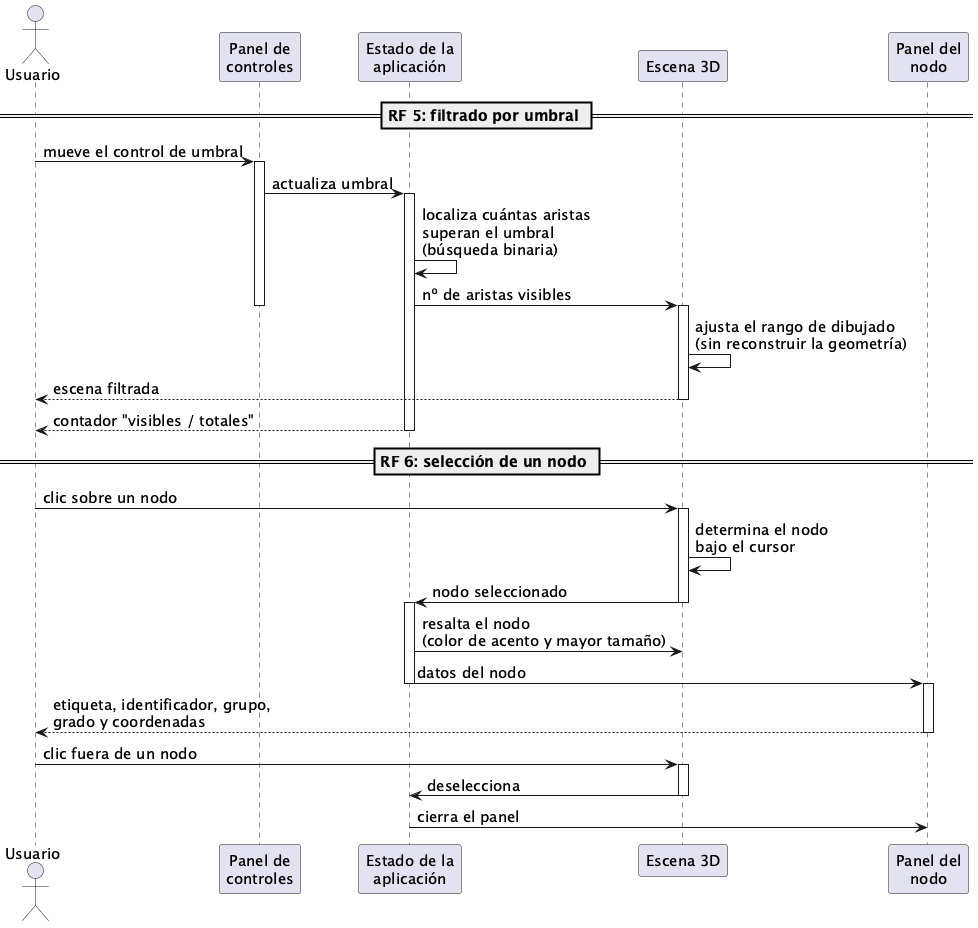
\includegraphics[width=\textwidth]{imagenes/sec_interaccion_sprint2}
	\caption{Diagrama de secuencia del filtrado por umbral (RF 5) y de la selección de un nodo (RF 6).}
	\label{fig:sec-s2}
\end{figure}

En cuanto a la selección (RF 6), se aprovecha la detección de intersecciones (\textit{raycasting})
que ofrece la librería de renderizado: al hacer clic, se determina qué nodo se encuentra bajo el
cursor y su identificador se guarda en el estado de la aplicación. A partir de ahí, y gracias al
modelo declarativo, tanto el resaltado del nodo en la escena como la aparición del panel de
información son consecuencia automática de ese cambio de estado. La deselección se resuelve
capturando los clics que no impactan sobre ningún nodo.

\subsection{Implementación}

\subsubsection*{Backend: red completa, grado y rango de pesos (RF 5, RF 6)}

En el módulo de parseo se ha eliminado el umbral fijo y se ha añadido el cálculo del grado. Como las
aristas de peso nulo no representan conexiones reales, se eliminan del grafo antes de calcular los
grados, de modo que el grado obtenido sea el correcto:

\begin{lstlisting}[language=Python, basicstyle=\footnotesize\ttfamily, keywordstyle=\color{blue!60!black}, commentstyle=\color{gray}, showstringspaces=false, frame=single, columns=fullflexible]
# Las aristas de peso nulo no representan conexion: se eliminan del grafo
# para que el grado de cada nodo sea el real
sin_conexion = [(u, v) for u, v, w in G.edges(data='weight') if w <= MIN_WEIGHT]
G.remove_edges_from(sin_conexion)

# Grado de cada nodo en la red completa (RF 6)
"degree": int(G.degree(i)),

# Aristas ordenadas por peso descendente: permite el filtrado eficiente (RF 5)
links_data.sort(key=lambda link: link["value"], reverse=True)
\end{lstlisting}

Se ha reforzado además la validación de los ficheros de entrada, comprobando que la matriz de
adyacencia sea cuadrada y que su dimensión coincida con el número de nodos declarados, y devolviendo
un error descriptivo en caso contrario [RNF 3].

\subsubsection*{Frontend: filtrado en tiempo real (RF 5)}

El componente de visualización construye la geometría una única vez y aplica el umbral ajustando el
rango de dibujado, siguiendo la estrategia descrita en el diseño:

\begin{lstlisting}[language=JavaScript, basicstyle=\footnotesize\ttfamily, keywordstyle=\color{blue!60!black}, commentstyle=\color{gray}, showstringspaces=false, frame=single, columns=fullflexible]
// Las aristas llegan ordenadas por peso: las visibles son siempre las
// primeras, asi que basta con ajustar el rango de dibujado (2 vertices/arista)
useEffect(() => {
  if (linesGeometry) linesGeometry.setDrawRange(0, settings.visibleLinks * 2);
}, [linesGeometry, settings.visibleLinks]);
\end{lstlisting}

El número de aristas visibles se obtiene con la búsqueda binaria descrita en el diseño, y alimenta
tanto la escena como el contador \textit{visibles / totales} del panel de estadísticas:

\begin{lstlisting}[language=JavaScript, basicstyle=\footnotesize\ttfamily, keywordstyle=\color{blue!60!black}, commentstyle=\color{gray}, showstringspaces=false, frame=single, columns=fullflexible]
// Posicion de la primera arista que ya no alcanza el umbral: O(log E)
function contarVisibles(links, umbral) {
  let ini = 0, fin = links.length;
  while (ini < fin) {
    const medio = (ini + fin) >> 1;
    if (links[medio].value >= umbral) ini = medio + 1;
    else fin = medio;
  }
  return ini;
}
\end{lstlisting}

\subsubsection*{Frontend: selección e inspección de nodos (RF 6)}

Cada nodo responde al evento de clic registrando su índice en el estado; volver a pulsar sobre el
mismo nodo lo deselecciona, y un clic fuera de cualquier nodo cierra la selección. El nodo
seleccionado se resalta con el color de acento de la interfaz y un tamaño mayor, mientras que el panel
muestra su etiqueta anatómica, identificador, grupo, grado y coordenadas.

Las figuras~\ref{fig:s2-umbral} y~\ref{fig:s2-seleccion} muestran el resultado de la implementación
sobre la red de ejemplo: la primera compara la red completa con la red filtrada, y la segunda recoge
la selección de una región con su panel de información.

\begin{figure}[H]
	\centering
	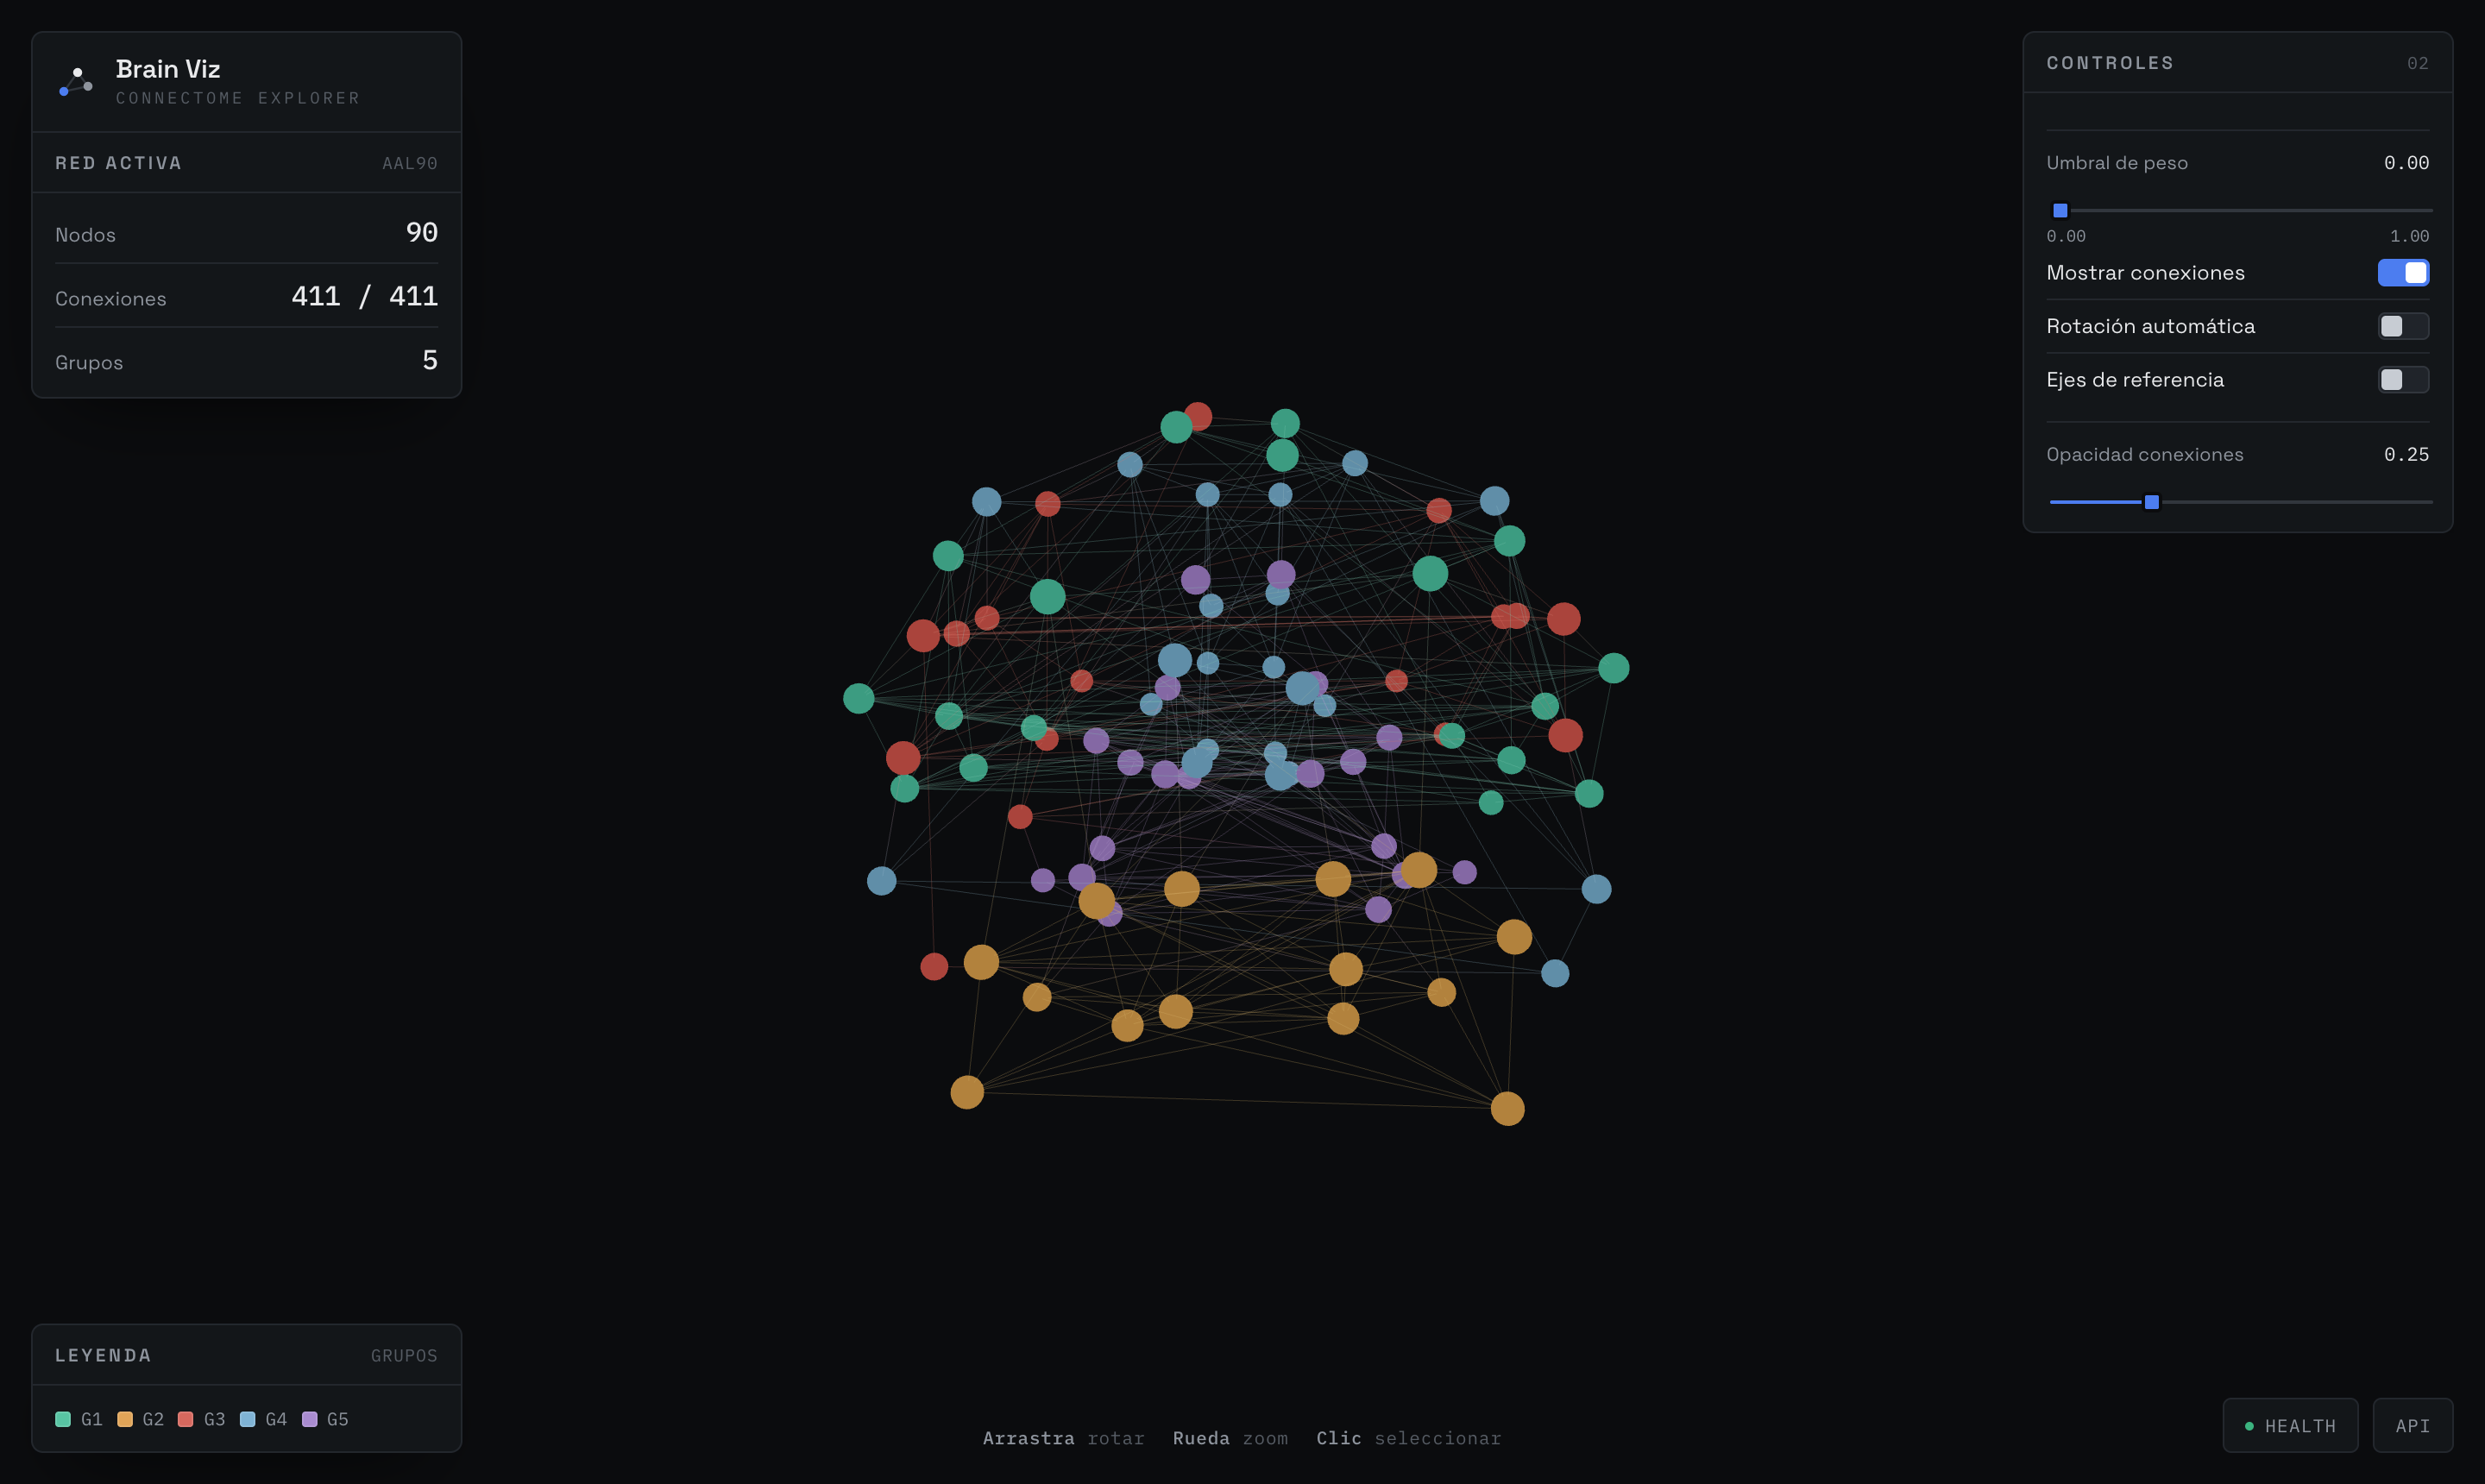
\includegraphics[width=0.86\textwidth]{imagenes/app_s2_umbral_bajo}\\[6pt]
	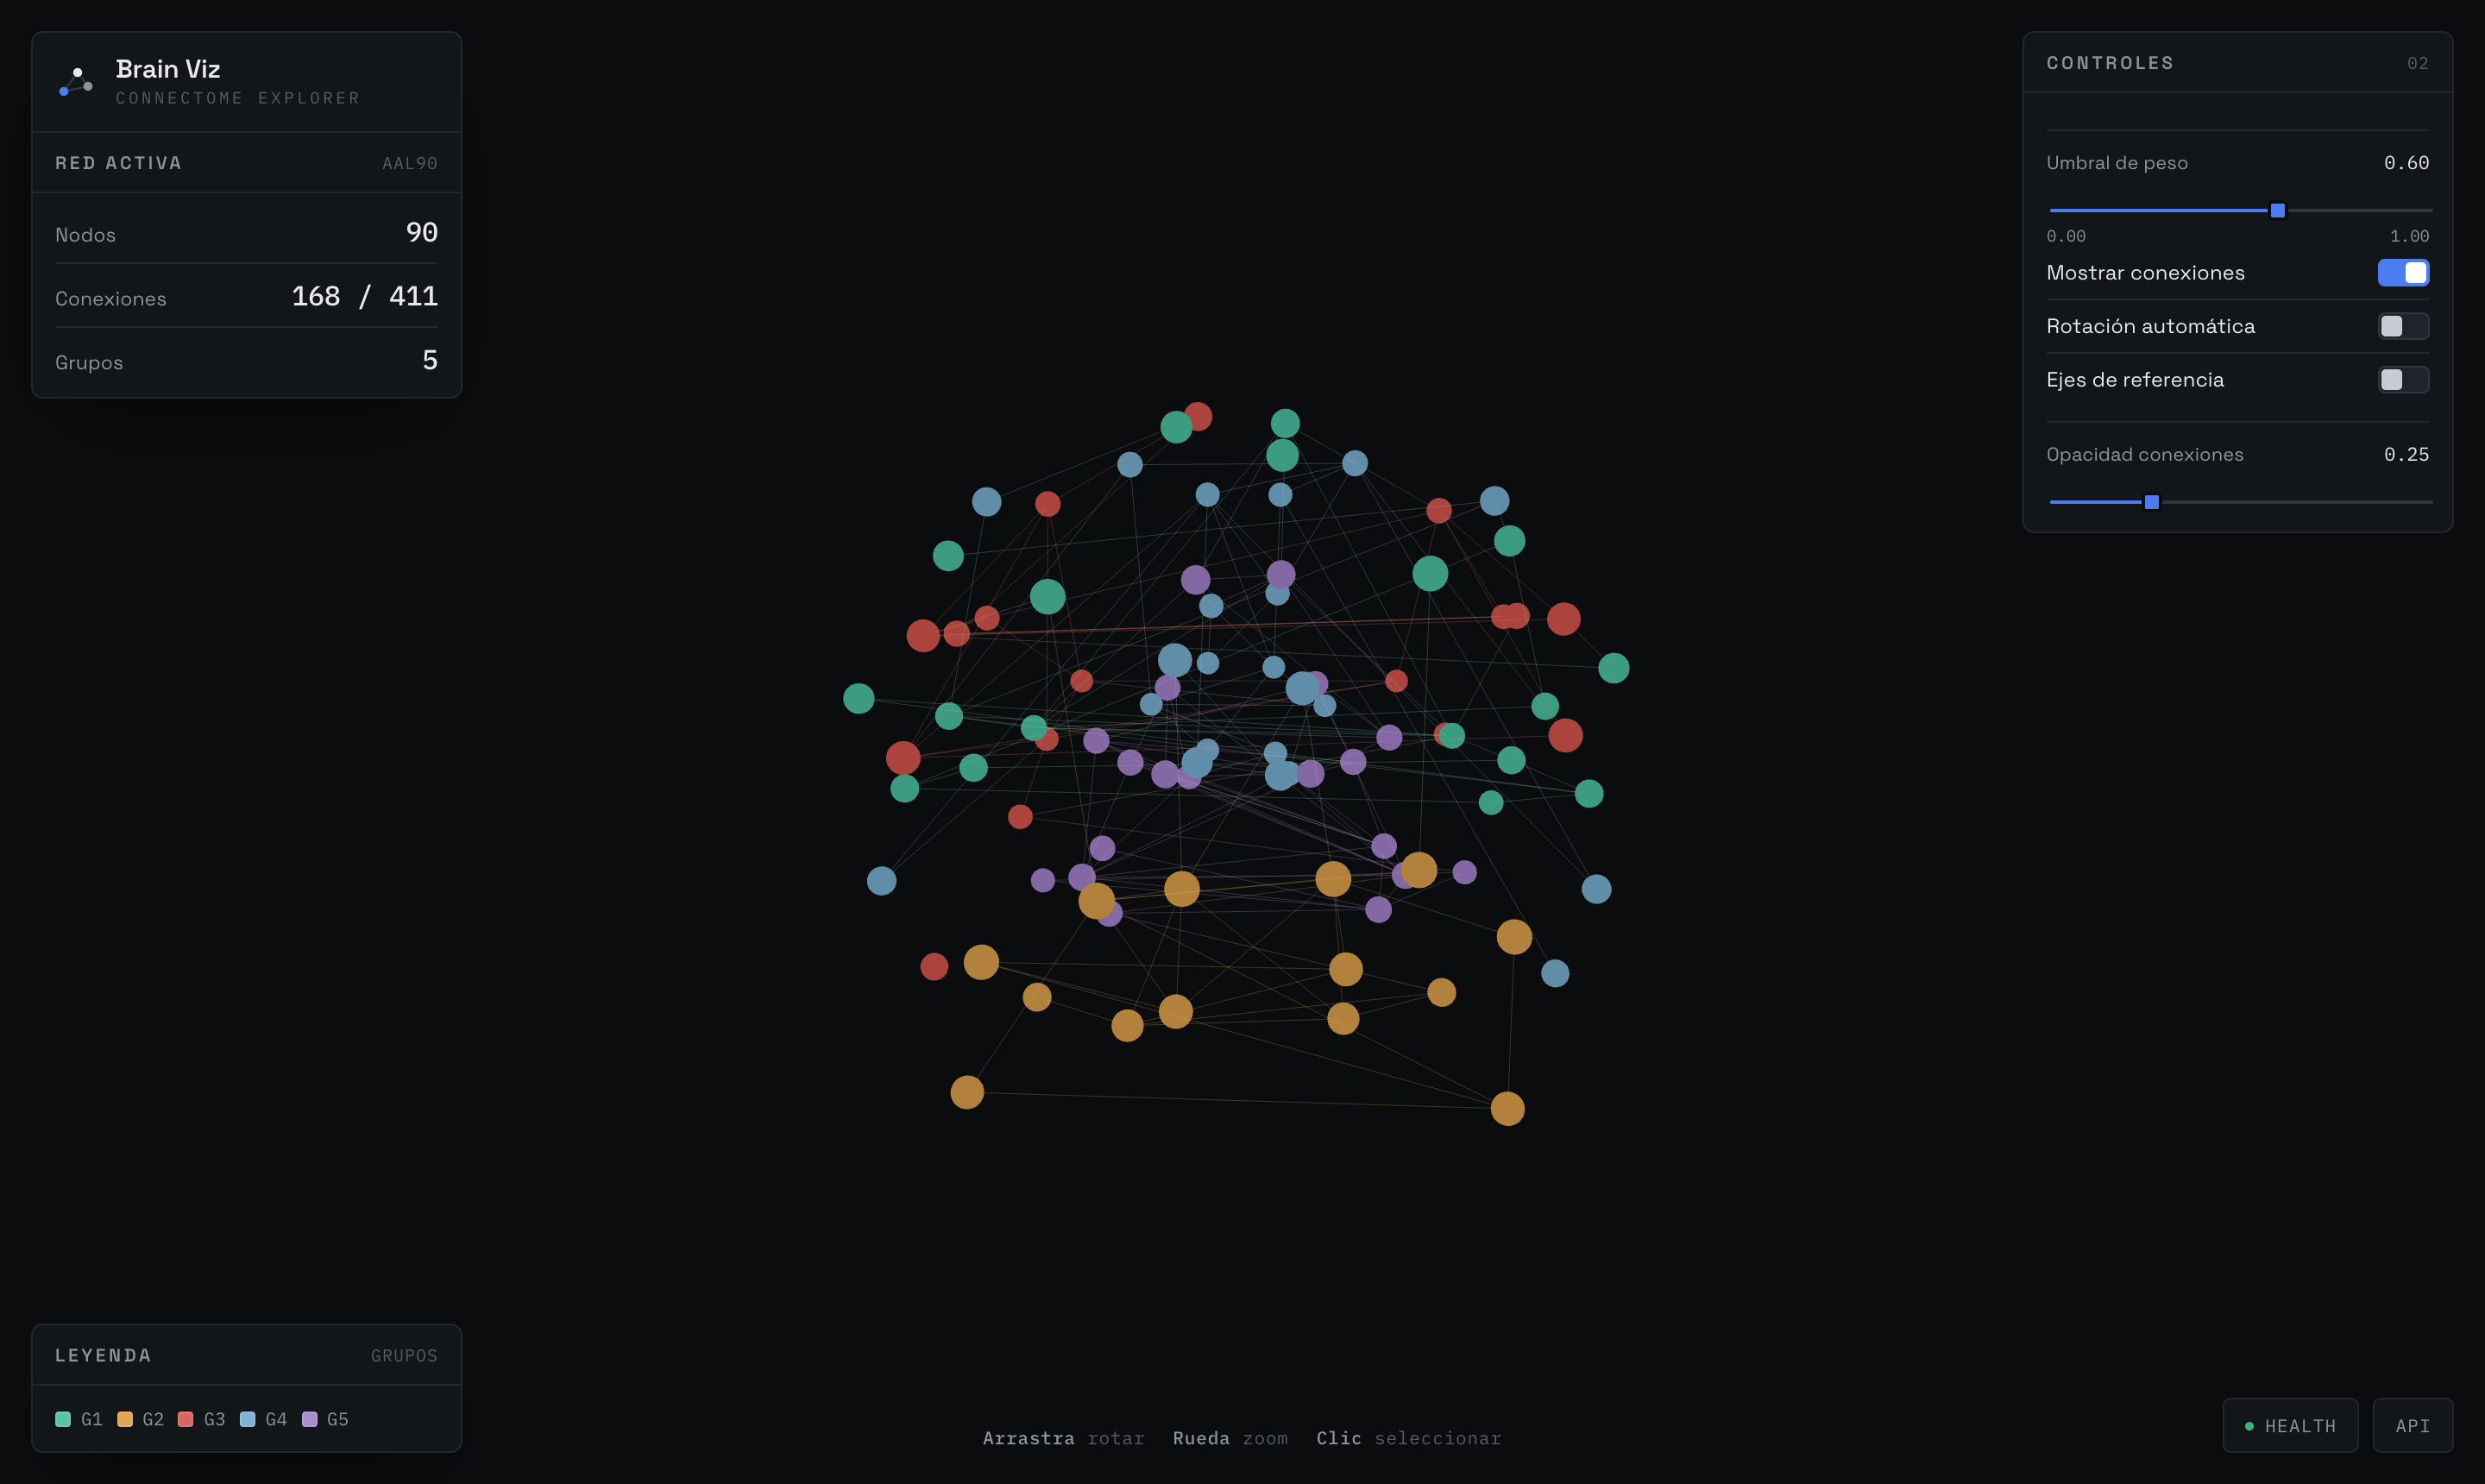
\includegraphics[width=0.86\textwidth]{imagenes/app_s2_umbral_alto}
	\caption{Filtrado por umbral (RF 5). Arriba: umbral 0,00, se muestran las 411 conexiones de la
	red. Abajo: umbral 0,60, quedan 168 conexiones y la estructura de la red se aprecia con mayor
	claridad. El contador del panel de estadísticas refleja en ambos casos la relación
	\textit{visibles / totales}.}
	\label{fig:s2-umbral}
\end{figure}

\begin{figure}[H]
	\centering
	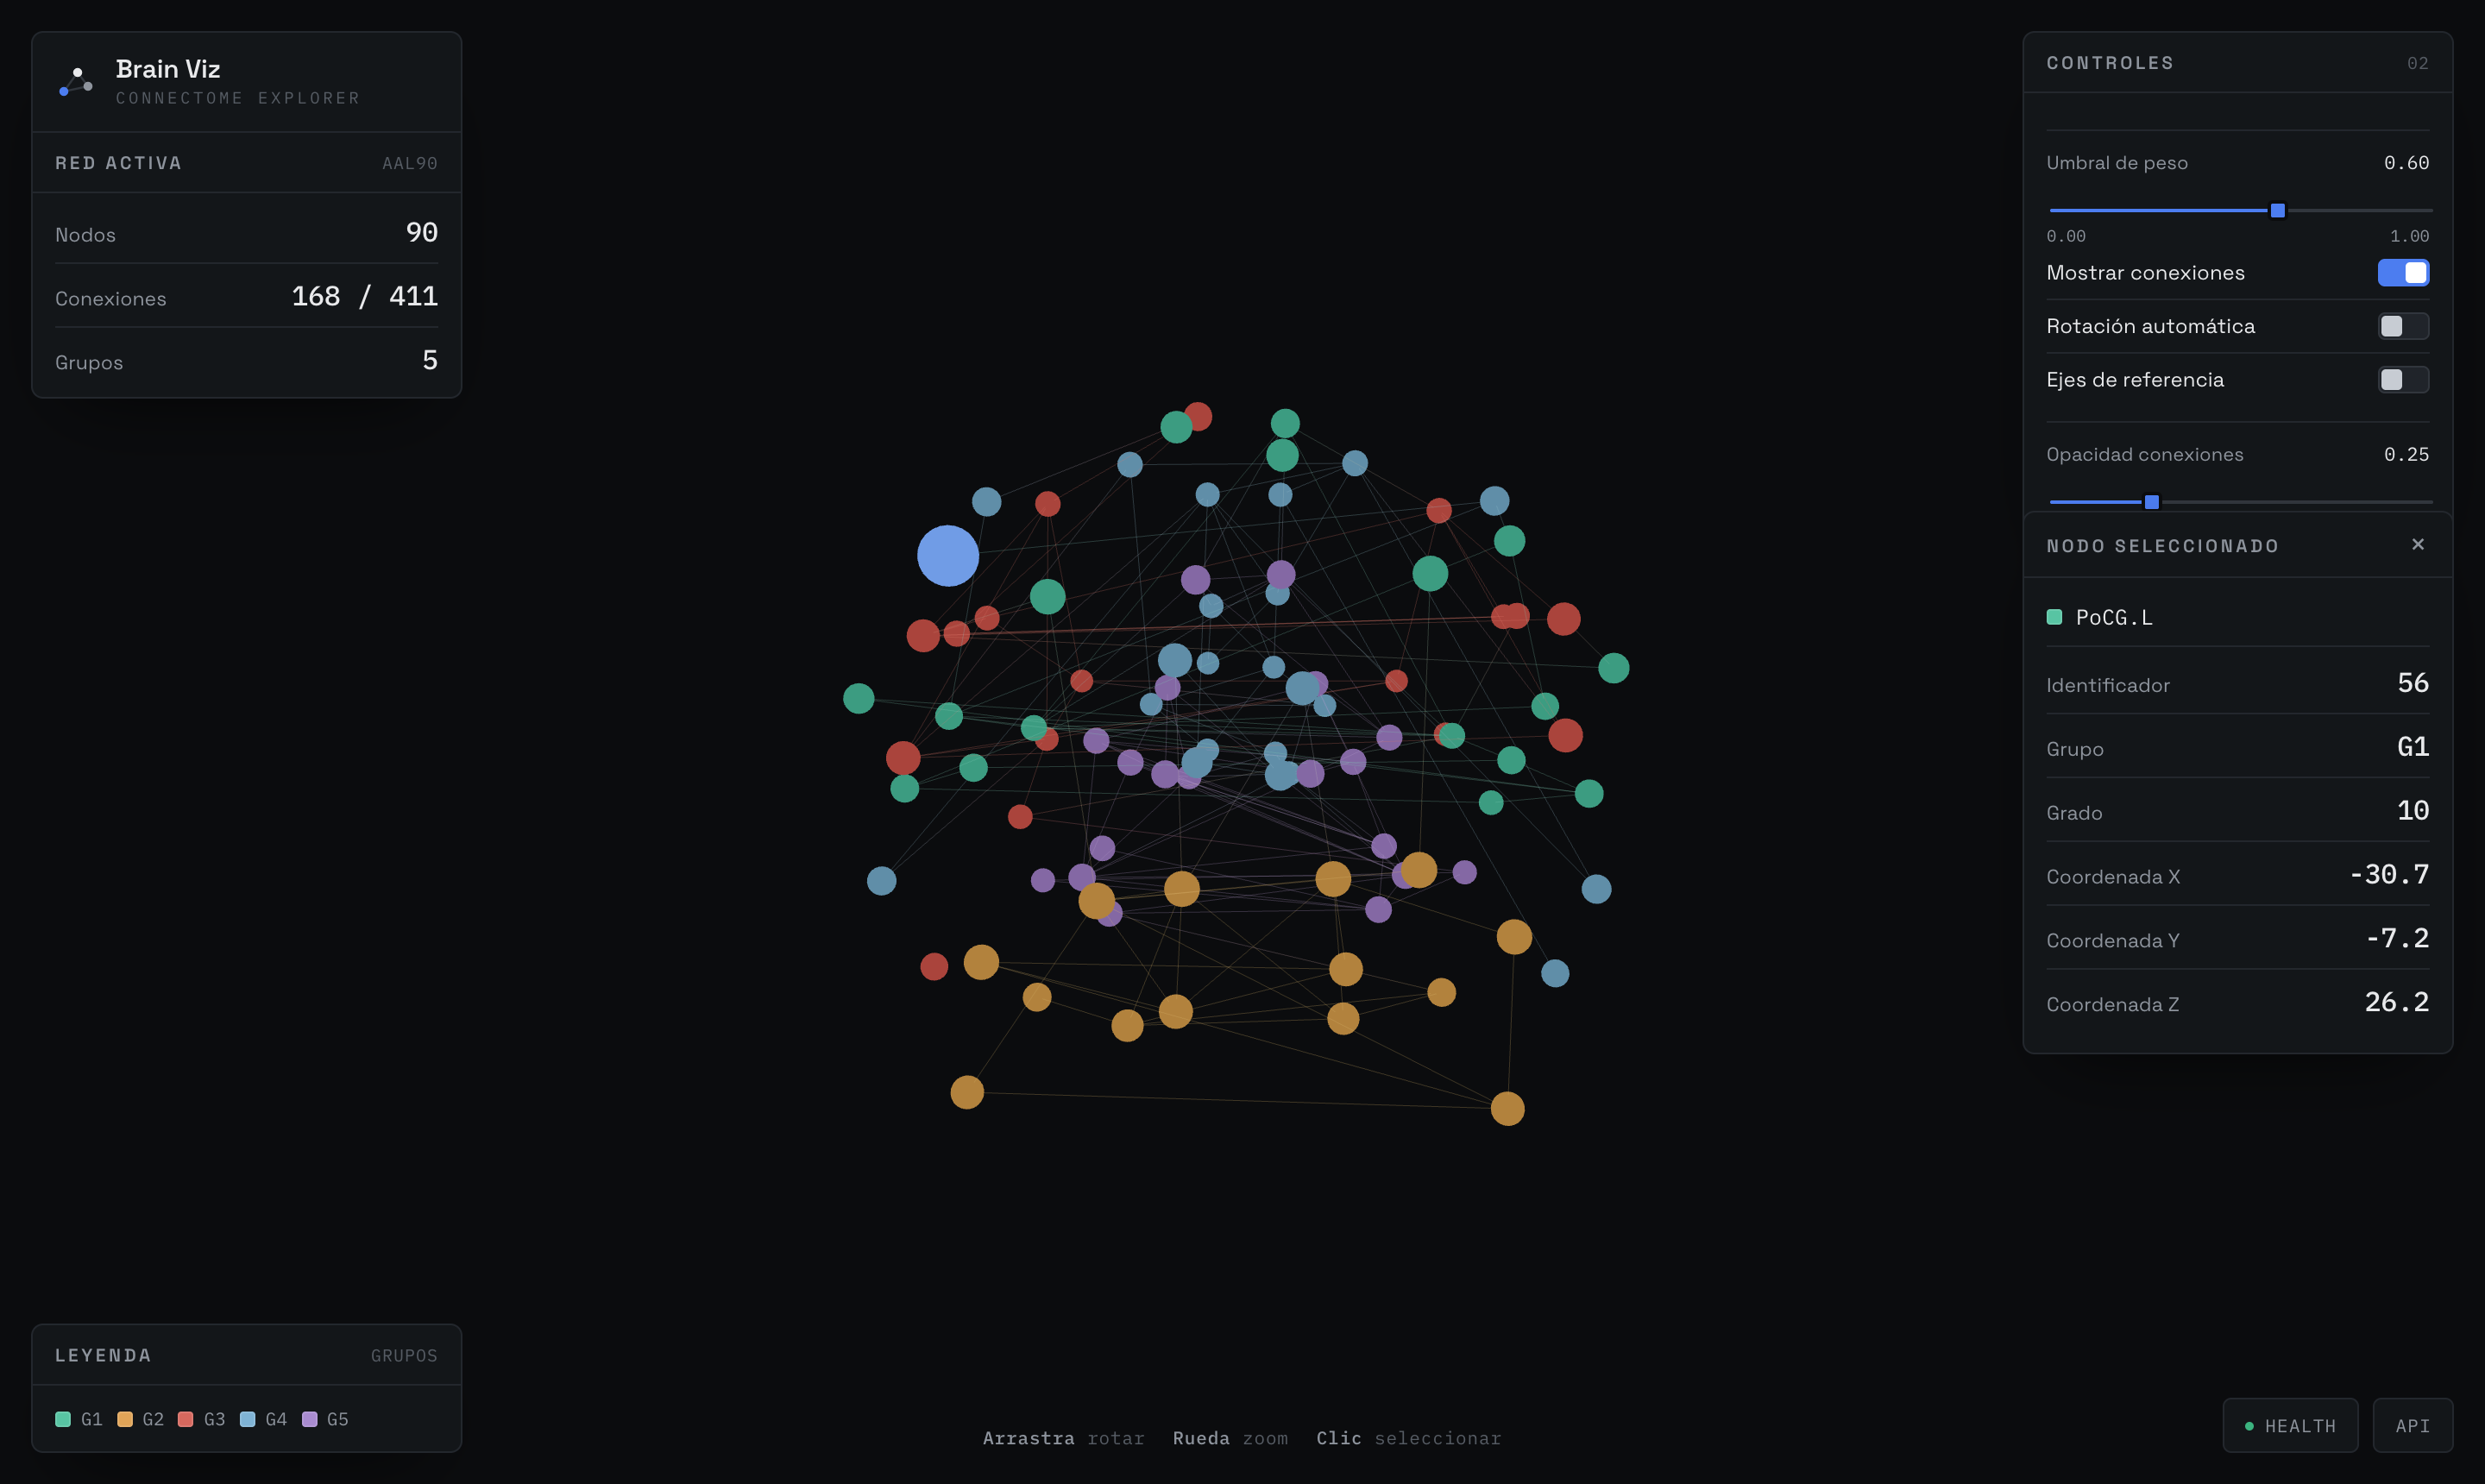
\includegraphics[width=\textwidth]{imagenes/app_s2_seleccion}
	\caption{Selección e inspección de un nodo (RF 6): la región \texttt{PoCG.L} aparece resaltada en la
	escena y el panel lateral muestra su identificador, grupo, grado y coordenadas.}
	\label{fig:s2-seleccion}
\end{figure}

\subsection{Pruebas}

Siguiendo la estrategia establecida en el \textit{sprint} anterior, las pruebas combinan caja blanca,
caja negra y validación.

\subsubsection*{Pruebas de caja blanca (unitarias)}

Se ha comprobado sobre el módulo de parseo que: el número de aristas devueltas coincide con el de
pares con peso no nulo de la matriz (411 en la red de ejemplo); la lista de aristas está efectivamente
ordenada de mayor a menor peso; el rango de pesos declarado en los metadatos coincide con el mínimo y
el máximo reales; y se cumple la identidad $\sum_i \text{grado}(i) = 2 \cdot |A|$, que verifica la
coherencia entre los grados calculados y el número de aristas. También se han probado los casos de
error: ficheros inexistentes, matriz no cuadrada y matriz cuyas dimensiones no coinciden con el número
de nodos.

\subsubsection*{Pruebas de caja negra (de integración)}

Se ha verificado que la respuesta de la API respeta el contrato ampliado, comprobando que cada nodo
incluye el atributo \texttt{degree} y que los metadatos incorporan \texttt{min\_weight} y
\texttt{max\_weight}. Sobre la aplicación en ejecución se ha contrastado que el contador de aristas
visibles que muestra la interfaz coincide, para distintos umbrales, con el número de aristas que
superan ese peso según los datos servidos por la API.

\subsubsection*{Pruebas de validación (de aceptación)}

La tabla~\ref{tab:pruebas-s2} recoge las pruebas de validación de los requisitos de este
\textit{sprint} y su resultado.

\begin{table}[H]
	\centering
	\caption{Pruebas de validación del Sprint 2.}
	\label{tab:pruebas-s2}
	\small
	\begin{tabularx}{\textwidth}{>{\raggedright\arraybackslash}p{1.5cm} >{\raggedright\arraybackslash}X >{\raggedright\arraybackslash}X >{\centering\arraybackslash}p{1.6cm}}
		\toprule
		\textbf{Prueba} & \textbf{Descripción} & \textbf{Resultado esperado} & \textbf{Estado} \\
		\midrule
		P-06 (RF 5) & Mover el control de umbral y observar la escena. &
			Las conexiones por debajo del umbral desaparecen de forma inmediata, sin esperas
			perceptibles. & Correcto \\
		\addlinespace
		P-07 (RF 5) & Comprobar el contador \textit{visibles / totales}. &
			Con umbral 0,50 se muestran 209 de 411 conexiones, cifra que coincide con el recuento sobre
			los datos de la API. & Correcto \\
		\addlinespace
		P-08 (RF 6) & Hacer clic sobre un nodo. &
			El nodo queda resaltado y se abre el panel con su etiqueta, identificador, grupo, grado y
			coordenadas. & Correcto \\
		\addlinespace
		P-09 (RF 6) & Contrastar el grado mostrado con el de la red. &
			El grado del panel coincide con el número de conexiones del nodo en los datos servidos. &
			Correcto \\
		\addlinespace
		P-10 (RF 6) & Hacer clic fuera de un nodo y pulsar el botón de cierre. &
			En ambos casos el nodo se deselecciona y el panel se cierra. & Correcto \\
		\addlinespace
		P-11 (RF 7) & Comprobar el coloreado por grupo y la leyenda. &
			Los nodos de un mismo grupo comparten color y la leyenda recoge los 5 grupos presentes. &
			Correcto \\
		\bottomrule
	\end{tabularx}
\end{table}

\subsubsection*{Pruebas de rendimiento (RNF 1)}

Una vez implementada la interacción, se ha abordado la comprobación del requisito no funcional de
fluidez [RNF 1]. Para poder evaluar el comportamiento con redes mayores que la de ejemplo, se ha
generado además una \textbf{red sintética de 500 nodos y 12.470 aristas} ---unas treinta veces más
conexiones que AAL90---, próxima al tamaño de referencia que fija el requisito. La medición se ha
realizado con un navegador controlado de forma automatizada, activando la rotación automática para
forzar un renderizado continuo (caso más desfavorable) y midiendo los intervalos entre fotogramas.
La tabla~\ref{tab:rendimiento} recoge los resultados.

\begin{table}[H]
	\centering
	\caption{Medición del rendimiento gráfico.}
	\label{tab:rendimiento}
	\small
	\begin{tabularx}{\textwidth}{>{\raggedright\arraybackslash}X >{\centering\arraybackslash}p{2.2cm} >{\centering\arraybackslash}p{2.2cm} >{\centering\arraybackslash}p{2.6cm}}
		\toprule
		\textbf{Red} & \textbf{Nodos} & \textbf{Aristas} & \textbf{Fotogramas/s} \\
		\midrule
		AAL90 (red de ejemplo)      & 90  & 411    & 30 \\
		Red sintética de prueba     & 500 & 12.470 & 30 \\
		\addlinespace
		\textit{Página vacía (referencia del entorno)} & --- & --- & \textit{30} \\
		\bottomrule
	\end{tabularx}
\end{table}

La interpretación de estos datos exige una precaución importante: al medir una \textbf{página vacía}
en el mismo entorno se obtiene también 30~fotogramas por segundo, lo que revela que es el propio
entorno de medida automatizado el que limita la tasa a ese valor. Por tanto, la medición
\emph{no permite verificar el objetivo de 60~FPS}, ya que ese techo no procede de la aplicación.

Lo que sí puede afirmarse es que la aplicación \textbf{sostiene el máximo que permite el entorno en
ambos casos}: multiplicar por treinta el número de aristas no produce ninguna degradación medible,
lo que indica que el renderizado no constituye un cuello de botella en el rango de tamaños
evaluado. Este resultado es coherente con la estrategia de diseño adoptada, que mantiene una única
geometría para todas las aristas y evita reconstruirla al filtrar. La verificación formal del
objetivo de $\geq 60$~FPS queda pendiente de realizarse con el perfilador de rendimiento de un
navegador de escritorio, y su resultado ---se alcance o no el objetivo--- se documentará en la
memoria final.

\subsubsection*{Errores detectados y corregidos}

Durante las pruebas de este \textit{sprint} se detectaron los siguientes errores:

\begin{itemize}
	\item \textbf{Grado incorrecto por aristas de peso nulo.} La primera versión calculaba el grado
		sobre el grafo construido directamente desde la matriz de adyacencia. Al comprobar la identidad
		$\sum_i \text{grado}(i) = 2 \cdot |A|$ se observó que no se cumplía: la librería creaba una
		arista por cada celda de la matriz, incluidas las de peso cero, de modo que todos los nodos
		presentaban el mismo grado (89, todos conectados con todos). Se corrigió eliminando del grafo
		las aristas de peso nulo antes de calcular los grados.
	\item \textbf{La deselección no cerraba el panel.} Durante la prueba automatizada, un clic en una
		zona aparentemente vacía no cerraba el panel de información. Al investigarlo se comprobó que el
		clic impactaba en realidad sobre el panel de la leyenda, superpuesto al lienzo, y que la
		deselección sí funcionaba al pulsar sobre una región libre de la escena. El error estaba en la
		prueba y no en la aplicación, pero el caso se documenta porque obligó a delimitar con precisión
		las zonas interactivas de la interfaz.
\end{itemize}

\subsubsection*{Validación por parte del cliente}

Al igual que en el \textit{sprint} anterior, la validación final corresponde al director del proyecto.
Para hacerla posible, la aplicación se ha \textbf{desplegado en un servidor accesible desde Internet},
de modo que tanto el director como, más adelante, los miembros del tribunal puedan probarla sin
instalar nada.

El despliegue emplea una \textbf{imagen de producción} distinta de la utilizada en desarrollo: en
lugar de dos servicios comunicados por un \textit{proxy} interno, se genera un único contenedor en el
que la interfaz de React se compila a ficheros estáticos y es servida por el propio \textit{backend}
mediante un servidor WSGI de producción. Esta decisión simplifica el despliegue, elimina la
dependencia de la red interna de contenedores y evita ejecutar servidores de desarrollo ---o el modo
de depuración--- en una dirección pública. El procedimiento completo se detalla en el manual de
instalación.
% NOTA: insertar aquí la URL pública del despliegue.
